\chapter{Discrete Probability and Counting}


\section{Introduction to Discrete Probability}
In a game of Monopoly, why do players land on the orange properties so
often? How many different ways can your class line up for a photo? What
are the odds that your phone's 4-digit passcode is guessed on the first
try? All of these are counting problems in disguise, and this chapter
gives you the tools to solve them.

Before we begin talking about discrete probability, let us address the word \emph{discrete}. It means ``individually
separate and distinct'' as in ``You can think of light as a
continuous wave or as a blast of discrete particles.''

When we are talking about probabilities, some problems deal
with discrete quantities like ``What is the probability that I will
throw these three dice and the numbers that roll face up sum to 9?'' There
are also problems that deal with continuous properties like ``What is
the probability that the next bird to fly over my house will weigh
between 97.2 and 98.1 grams?'' In this module, we are going to focus
on the probability problems that deal with discrete quantities.

Watch Khan Academy's Introduction to Probability at \url{https://youtu.be/uzkc-qNVoOk}.

Let us say that you have a cloth sack filled with 100 marbles; 99 are red
and 1 is white. If you reach in without looking and pull out
one marble, you will probably pull out a red one. We say that ``There
is a 1 in 100 chance that you would pull out a white marble.'' Or we
can use percentages and say ``There is a 1\% chance that you will pull
out a white marble.'' Or we can use decimals and say ``There is a 0.01
probability that you will pull out a white marble.''
% Bag Diagram
In probability, we often talk about the probability of certain
events. ``Pulling out a white marble'' is an event, and we can give it
a symbol like $W$. In equations, we use $p$ to mean ``the
probability of''. Thus, we can say ``There is a 0.01 probability that
you will pull out a white marble,'' which becomes the equation
\begin{equation*}
  p(W) = 0.01
\end{equation*}\index{probability}
% ADD: Make sure functions come before this chapter, connect to functions

\subsection{The Probability of All Possibilities is 1.0}\index{probability!sum to one}

We know that you are either going to pull out a red marble or a white marble,
so the probability of a white marble being pulled and the probability
of a red marble being pulled must add up to 100\%. Therefore, the probability of
pulling out a red marble must be 99\%, or 0.99. If we let the event ``Pull out a red marble'' be given by the symbol $R$, we can say:
\begin{equation*}
  p(R) = 1.0 - p(W) = 1.0 - 0.01 = 0.99
\end{equation*}

Now, let us say that you take a marble from the bag, then
toss a coin. What is the probability that you will pull a white marble, then get heads on the coin? It is the product of the two
probabilities: $0.01 \times 0.5 = 0.005$, so one-half of a one percent
chance. Do the probabilities still sum to 1?
\begin{itemize}
\item White and Heads = $0.01 \times 0.5 = 0.005$
\item White and Tails = $0.01 \times 0.5 = 0.005$
\item Red and Heads = $0.99 \times 0.5 = 0.495$
\item Red and Tails = $0.99 \times 0.5 = 0.495$
% ADD: add up the values at the end for clarity
\end{itemize}
$0.005 + 0.005 + 0.495 + 0.495 = 1.000$
Yes, the probabilities of all the possibilities still add to 1. We were allowed to multiply because \emph{the events do not affect each other}: the events are \textbf{\textit{independent}}. 
\subsection{Independence and Dependence}

In the last section, you learned that the probability of two events
(``Pulling a red marble from the bag'' and ``Getting tails in a coin
toss'') is the product of the probability of each event: $0.99 \times 0.5 = 0.495$.

This is true if the two events are \textit{independent}; that is, the
outcome of one does not change the probability of the other. The
example we gave is independent: It does not matter what ball you pull
from the bag, the outcome of the coin toss will always be 50-50.\index{independent event}

What is an example of two events that are not independent? The probability that a
person is a professional basketball player and the probability that
someone wears a shoe that is size 13 or larger is \textit{not}
independent; rather it is dependent. After all, height is an advantage in basketball, and most
tall people also have large feet. So, if you know someone is a
basketball player, they likely wear large shoes.
\index{dependent event}

\subsection{Correlation does not Imply Causation}
It is often said that ``Correlation does not imply causation''. What does this mean? 
\index{correlation and causation}
Breaking it down:
\begin{itemize}
  \item Correlation is a state in which two things increase or decrease together; two variables are \emph{linearly} related
  \item Imply means suggests, as in \textit{there is evidence for}
  \item Causation means there is a cause and effect relationship in place between the two variables. 
\end{itemize}

So saying correlation does not imply causation simply means: just because two variables are linearly connected, it cannot be said one variable causes the other. 

Here are some examples:
\begin{itemize}
  \item Ice Cream Sales, Mosquito bites, and Sunburn cases all increase during the summertime. However, none of them causes another: hot, sunny weather drives all three.
  \item Dinosaurs were not able to read books. However, this does not mean that the inability to read caused dinosaur extinction. 
  \item There was a large increase in toilet paper sales and people working from home in the years 2020-2021. Does this mean that one causes the other? Not necessarily. In this case a third factor $C$, the pandemic, caused a large global quarantine, leading to increased toilet paper usage and the inability to work in an office. 
\end{itemize}

% ADD: Correlation for Causation 
    % added a draft form Arjan 20Aug25
    % both links added to DR. 
% Weird Correlations Website: https://www.tylervigen.com/spurious-correlations
% KA: https://youtu.be/R-NeYKSEqns

\begin{Exercise}[title={Rolling Dice}, label=rolling-dice]
  If you have three six-sided dice to roll, what is the
  probability that you will roll a five on all three dice?
\end{Exercise}
\begin{Answer}[ref=rolling-dice]
  probability of all 5's $ = \frac{1}{6}\times\frac{1}{6}\times\frac{1}{6} = \left(\frac{1}{6}\right)^3 = \frac{1}{216} \approx 0.0046$
  \end{Answer}
    
\begin{Exercise}[title={Flipping Coins}, label=flipping-coins]
  If you have five coins to flip, what is the
  probability that at least one coin will come up heads?
\end{Exercise}
\begin{Answer}[ref=flipping-coins]
  probability of at least one heads = 1.0 - probability of all tails $ = 1.0 - \left(\frac{1}{2}\right)^5 =1.0 - \frac{1}{32} = \frac{31}{32} \approx 0.97$ 

  
\includegraphics[width=0.5\textwidth]{coin_prob.png}
\end{Answer}
    
\subsection{Why 7 is the most likely sum of two dice}\index{dice sum distribution}

If you roll two dice, the sum will be 2, 12, or any number in
between. It is very tempting to assume that the likelihood of any of
those numbers is the same. In fact, the probability of a 2 is
$\frac{1}{36} \approx 3\%$ and the probability of a 7 is $\frac{1}{6}
\approx 17\%$. A 7 is six times more likely than a 12! Why?

When you roll the first die, there are six possibilities with equal
probability. When you roll the second die, there are six possibilities
with equal probability. So, there are a total of 36 possible events
with equal probabilities: 1 then 1, 1 then 2, 2 then 1, 1 then 3, 3
then 1, and so on. Only one of these (1 then 1) adds to 2. However, six of these
sum to 7: 1 then 6, 6 then 1, 2 then 5, 5 then 2, 3 then 4, and 4 then
3. So, a 7 is six times more likely than a 2.

Here is the complete table:
%Dice Diagram
\begin{tabular}{c| c c c c c c | c | c}
  Sum &     &     &     &     &     &     & Count & Probability \\
  \hline
  2   & 1,1 &     &     &     &     &     &   1    & 1/36 \\
  3   & 1,2 & 2,1 &     &     &     &     &   2    & 1/18 \\
  4   & 1,3 & 2,2 & 3,1 &     &     &     &   3    & 1/12 \\
  5   & 1,4 & 2,3 & 3,2 & 4,1 &     &     &   4    & 1/9 \\
  6   & 1,5 & 2,4 & 3,3 & 4,2 & 5,1 &     &   5    & 5/36 \\
  7   & 1,6 & 2,5 & 3,4 & 4,3 & 5,2 & 6,1 &   6    & 1/6 \\
  8   &     & 2,6 & 3,5 & 4,4 & 5,3 & 6,2 &   5    & 5/36 \\
  9   &     &     & 3,6 & 4,5 & 5,4 & 6,3 &   4    & 1/9 \\
  10  &     &     &     & 4,6 & 5,5 & 6,4 &   3    & 1/12 \\
  11  &     &     &     &     & 5,6 & 6,5 &   2    & 1/18 \\
  12  &     &     &     &     &     & 6,6 &   1    & 1/36
\end{tabular}

If you do not believe these numbers, you could
roll a pair of dice hundreds of times and make a histogram. However, it would be a
tedious and time-consuming task --- just the sort of thing that we make
computers do for us.
% ADD: Define Histogram
% histogram is defined before this in the stats chapter - Arjan Aug25

\begin{figure}[H]
    \centering
    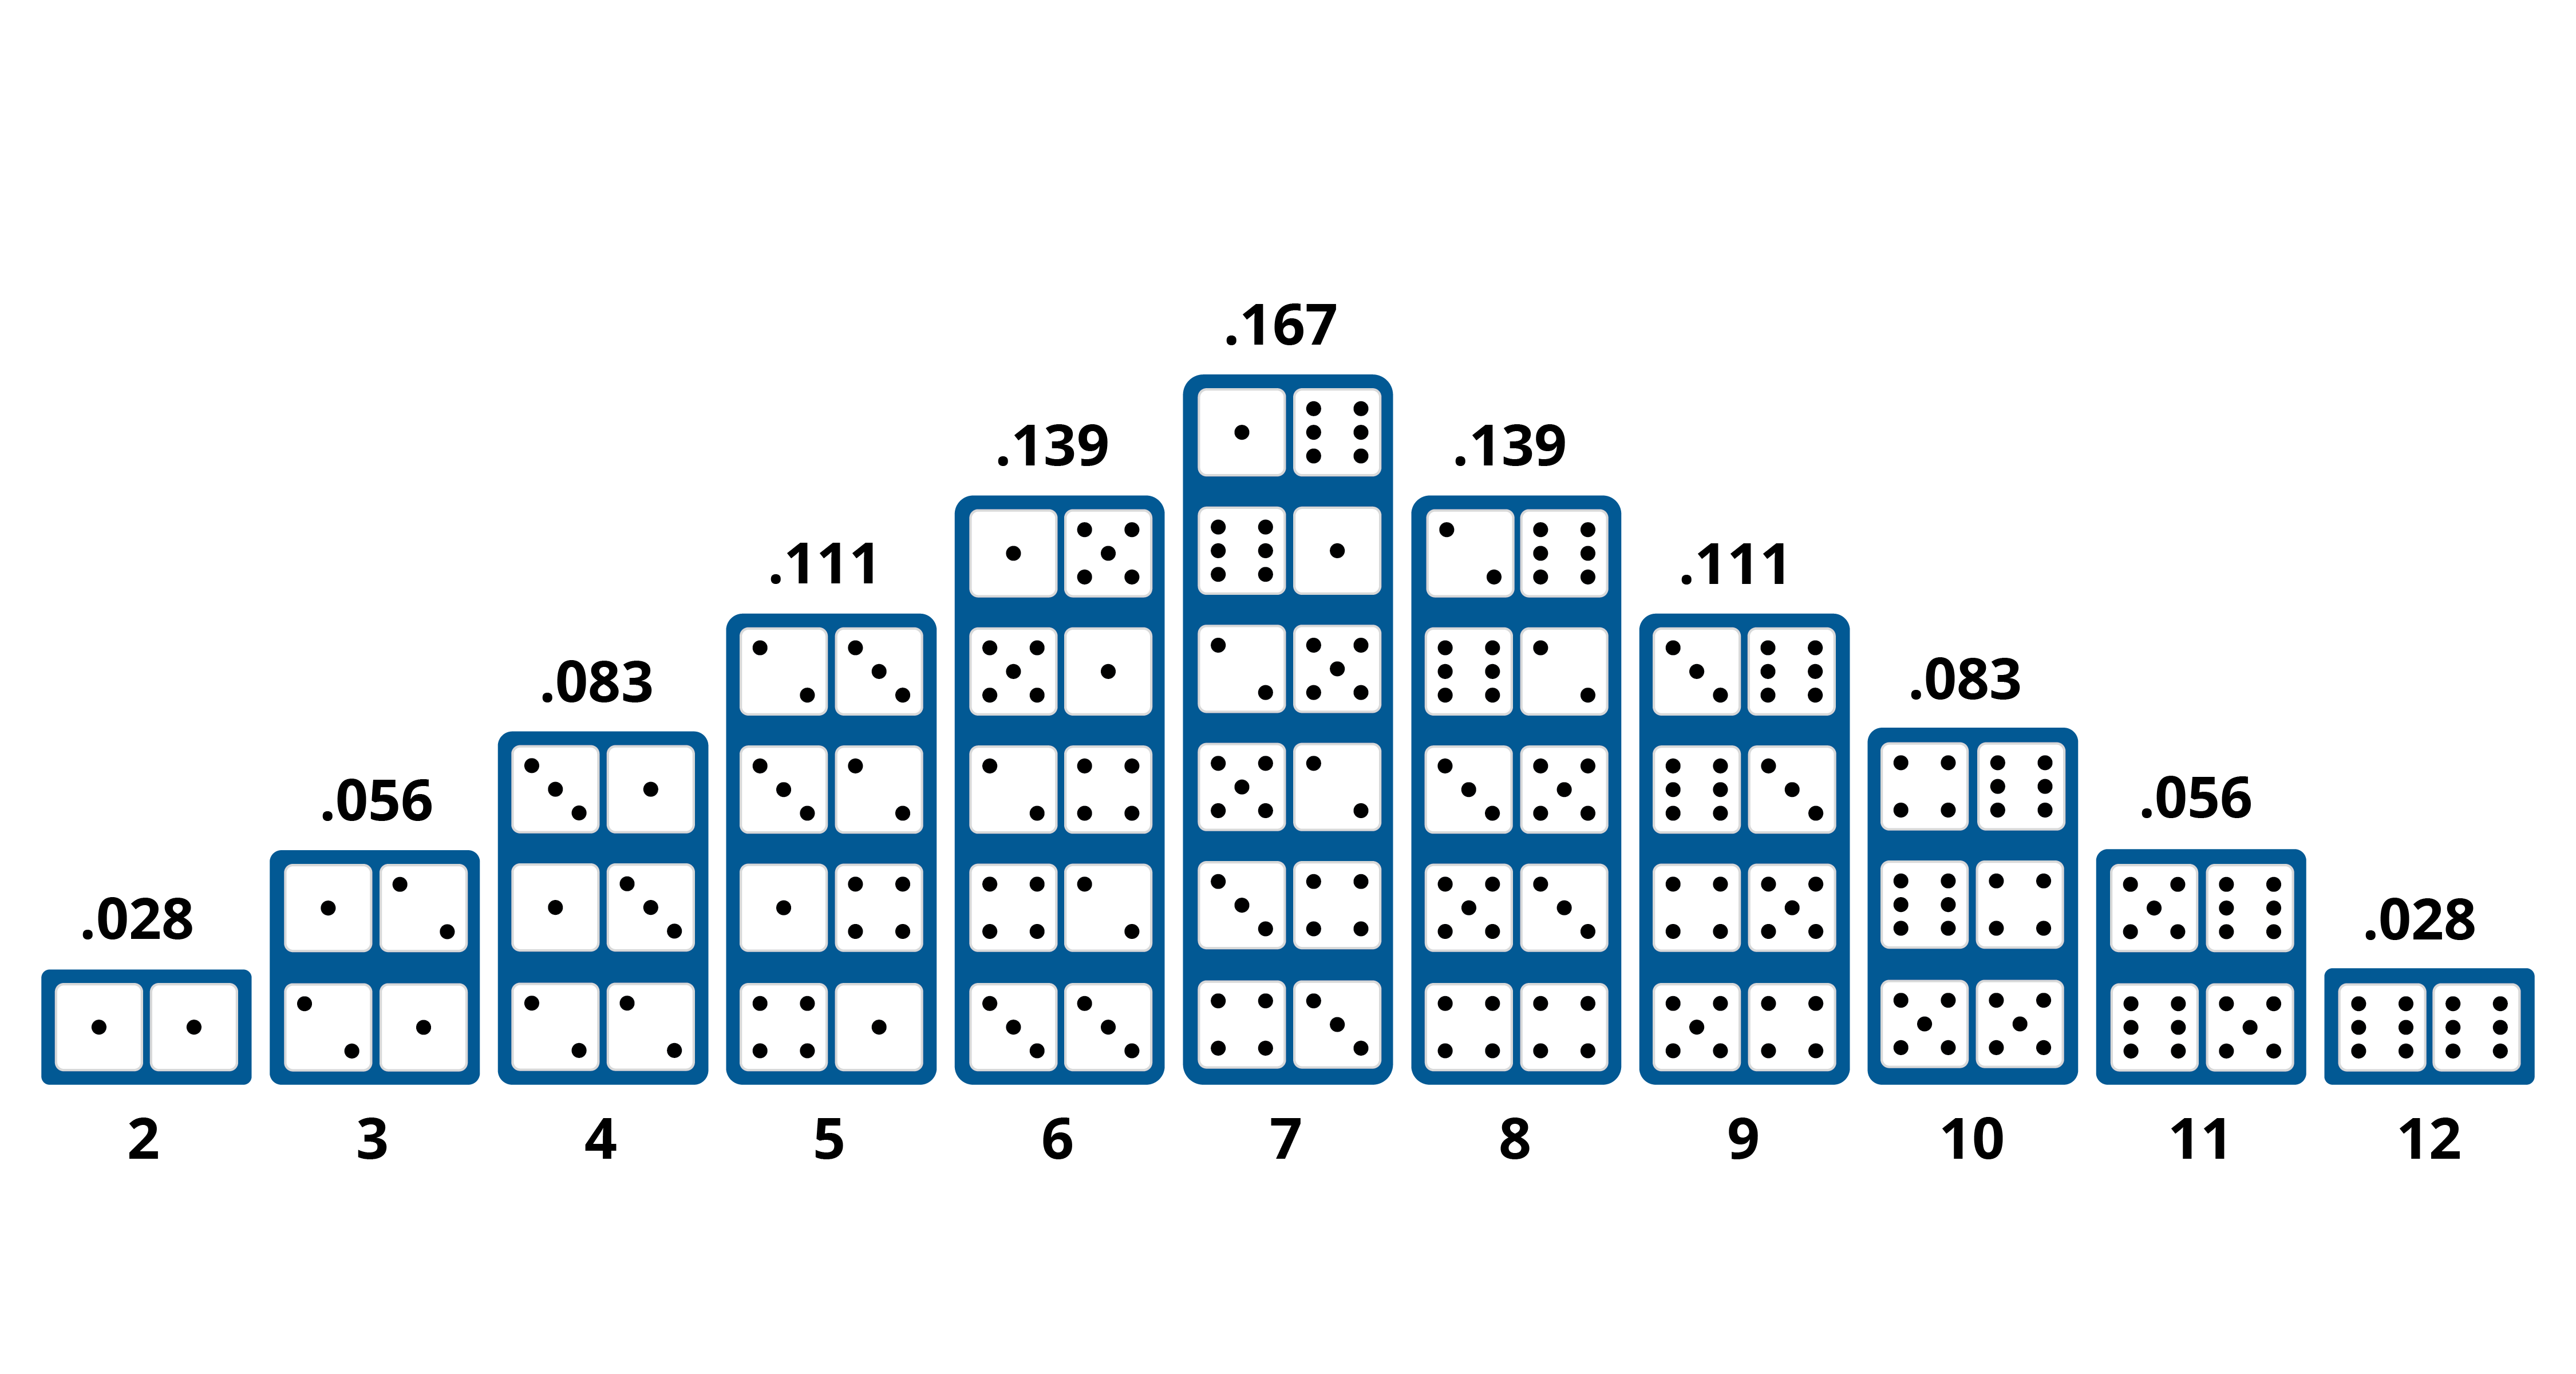
\includegraphics[width=1\textwidth]{dice_histogram.png}
    \caption{A histogram of probabilities of dice sums. With two dice, the shape is a triangle; with more dice, it gets closer and closer to a bell curve.}
    \label{fig:dice_histogram}
\end{figure}
\subsection{Random Numbers and Python}

You are going to write a \index{simulation}simulation of rolling dice in Python. To do
this, you will need to generate a random sequence of numbers. The
numbers will need to be in the range 1 to 6, and they will need to
appear in the sequence with the same frequency. We say the sequence
will follow \textit{the uniform distribution}. In other words, the
probability is uniformly distributed among the 6 possibilities.\index{random number generation}

Start python and try a few of the different ways to generate random numbers:
\begin{minted}{python}
> python3
>>> import random
>>> random.random()  # Generates a random floating point number between 0 and 1
0.6840892758539989
>>> random.randrange(5)      # Generates an integer in the range 0 - 4
2
>>> x = ['Rock', 'Paper', 'Scissors']
>>> random.choice(x)   # Pick a random entry from the sequence
'Paper'
>>> x
['Rock', 'Paper', 'Scissors'] 
>>> random.shuffle(x)   # Shuffle the order of the sequence
>>> x
['Scissors', 'Paper', 'Rock']
>>> a = list(range(30))
>>> a
[0, 1, 2, 3, 4, 5, 6, 7, 8, 9, 10, 11, 12, 13, 14, 15,
  16, 17, 18, 19, 20, 21, 22, 23, 24, 25, 26, 27, 28, 29]
>>> random.sample(a, 10) # Return 10 randomly chosen items from the sequence
[8, 7, 20, 9, 25, 13, 23, 11, 14, 16]
\end{minted}
% KA: https://www.youtube.com/watch?v=Jua-KWBdzfU
Clearly, Python has many ways to do things that look random. However, here is the hidden truth: they are not really
random. The computer that you are using cannot generate random
data. Instead, it uses tricks to create data that look random; we
call this \index{pseudorandom numbers}\textit{pseudorandom} data. Good pseudorandom algorithms are
very important for cryptography and data security.

What if you want real random data? Some companies are using
the decay of radioactive materials to generate real random data. You
can pay to download it. For our purposes, Python's pseudorandom
numbers are quite sufficient.

If we generate two random numbers in the range 1 through 6 and add them together, we
will have simulated rolling a pair of dice. Like this:

\begin{minted}{python}
>>> a = random.randrange(6) + 1
>>> b = random.randrange(6) + 1
>>> a + b
8
\end{minted}

First, let us write a program that just rolls the dice 100 times and shows the result. Make a file \filename{dice.py}:
\begin{minted}{python}
import random

roll_count = 100

for i in range(roll_count):
    a = random.randrange(6) + 1
    b = random.randrange(6) + 1
    roll = a + b
    print(f"Toss {i}: {a} + {b} = {roll}")
\end{minted}

When you run it, you should see something like:
\begin{minted}{python}
> python3 dice.py
Toss 0: 6 + 6 = 12
Toss 1: 4 + 4 = 8
Toss 2: 4 + 2 = 6
Toss 3: 4 + 6 = 10
Toss 4: 4 + 4 = 8
...
Toss 98: 5 + 2 = 7
Toss 99: 5 + 2 = 7
\end{minted}

Now we want to count occurrences of each possible outcome. Let us use an
array of integers. We will start with an array of zeros. When we roll a 3, we will add 1 to item 3 in the array. (We can
never roll a zero or a one, so those two entries will always be zero.)
% ADD: Define Array
\begin{minted}{python}
import random

roll_count = 100

# Make an array containing 13 zeros
counts = [0] * 13

for i in range(roll_count):
    a = random.randrange(6) + 1
    b = random.randrange(6) + 1
    roll = a + b
    print(f"Toss {i}: {a} + {b} = {roll}")

    # Increment the count for roll
    counts[roll] += 1

print(f"Counts: {counts}")
\end{minted}

When you run this, at the end you will see a count for each possible outcome:

\begin{minted}{python}
...
Toss 98: 3 + 2 = 5
Toss 99: 6 + 1 = 7
Counts: [0, 0, 2, 6, 16, 11, 13, 14, 11, 11, 6, 9, 1]
\end{minted}

\index{expected count}What was the count that we expected? For example, we expected to see a
2 about once every 36 rolls, right? It might be nice to compare our
count to what we expected. Add a few more lines, and we are going to
increase the number of rolls. You will probably want to delete the
line that prints each roll separately:

\begin{minted}{python}
import random

# Can't ever be 0 or 1
p = [0.0, 0.0, 1/36, 1/18, 1/12, 1/9, 5/36, 1/6, 5/36, 1/9, 1/12, 1/18, 1/36]
roll_count = 1000

# Make an array containing 13 zeros
counts = [0] * 13

for i in range(roll_count):
    a = random.randrange(6) + 1
    b = random.randrange(6) + 1
    roll = a + b

    # Increment the count for roll
    counts[roll] += 1

for i in range(2,13):
    print(f"{i} appeared {counts[i]} times, expected {p[i] * roll_count:.1f}")
\end{minted}

Now you should see something like:
\begin{minted}{python}
2 appeared 39 times, expected 27.8
3 appeared 55 times, expected 55.6
4 appeared 84 times, expected 83.3
5 appeared 110 times, expected 111.1
6 appeared 160 times, expected 138.9
7 appeared 176 times, expected 166.7
8 appeared 124 times, expected 138.9
9 appeared 93 times, expected 111.1
10 appeared 87 times, expected 83.3
11 appeared 49 times, expected 55.6
12 appeared 23 times, expected 27.8
\end{minted}

Whenever you are dealing with random numbers, the outcome will seldom
be \textit{exactly} what you expected. In this case, however, you should see that your
predictions are pretty close.

\subsubsection{Making a bar graph}



A bar graph is a nice way to look at quantities like this. Let us make a bar graph that shows the actual count and the expected count:\index{bar graph!in python}

\begin{figure}[H]
    \centering
    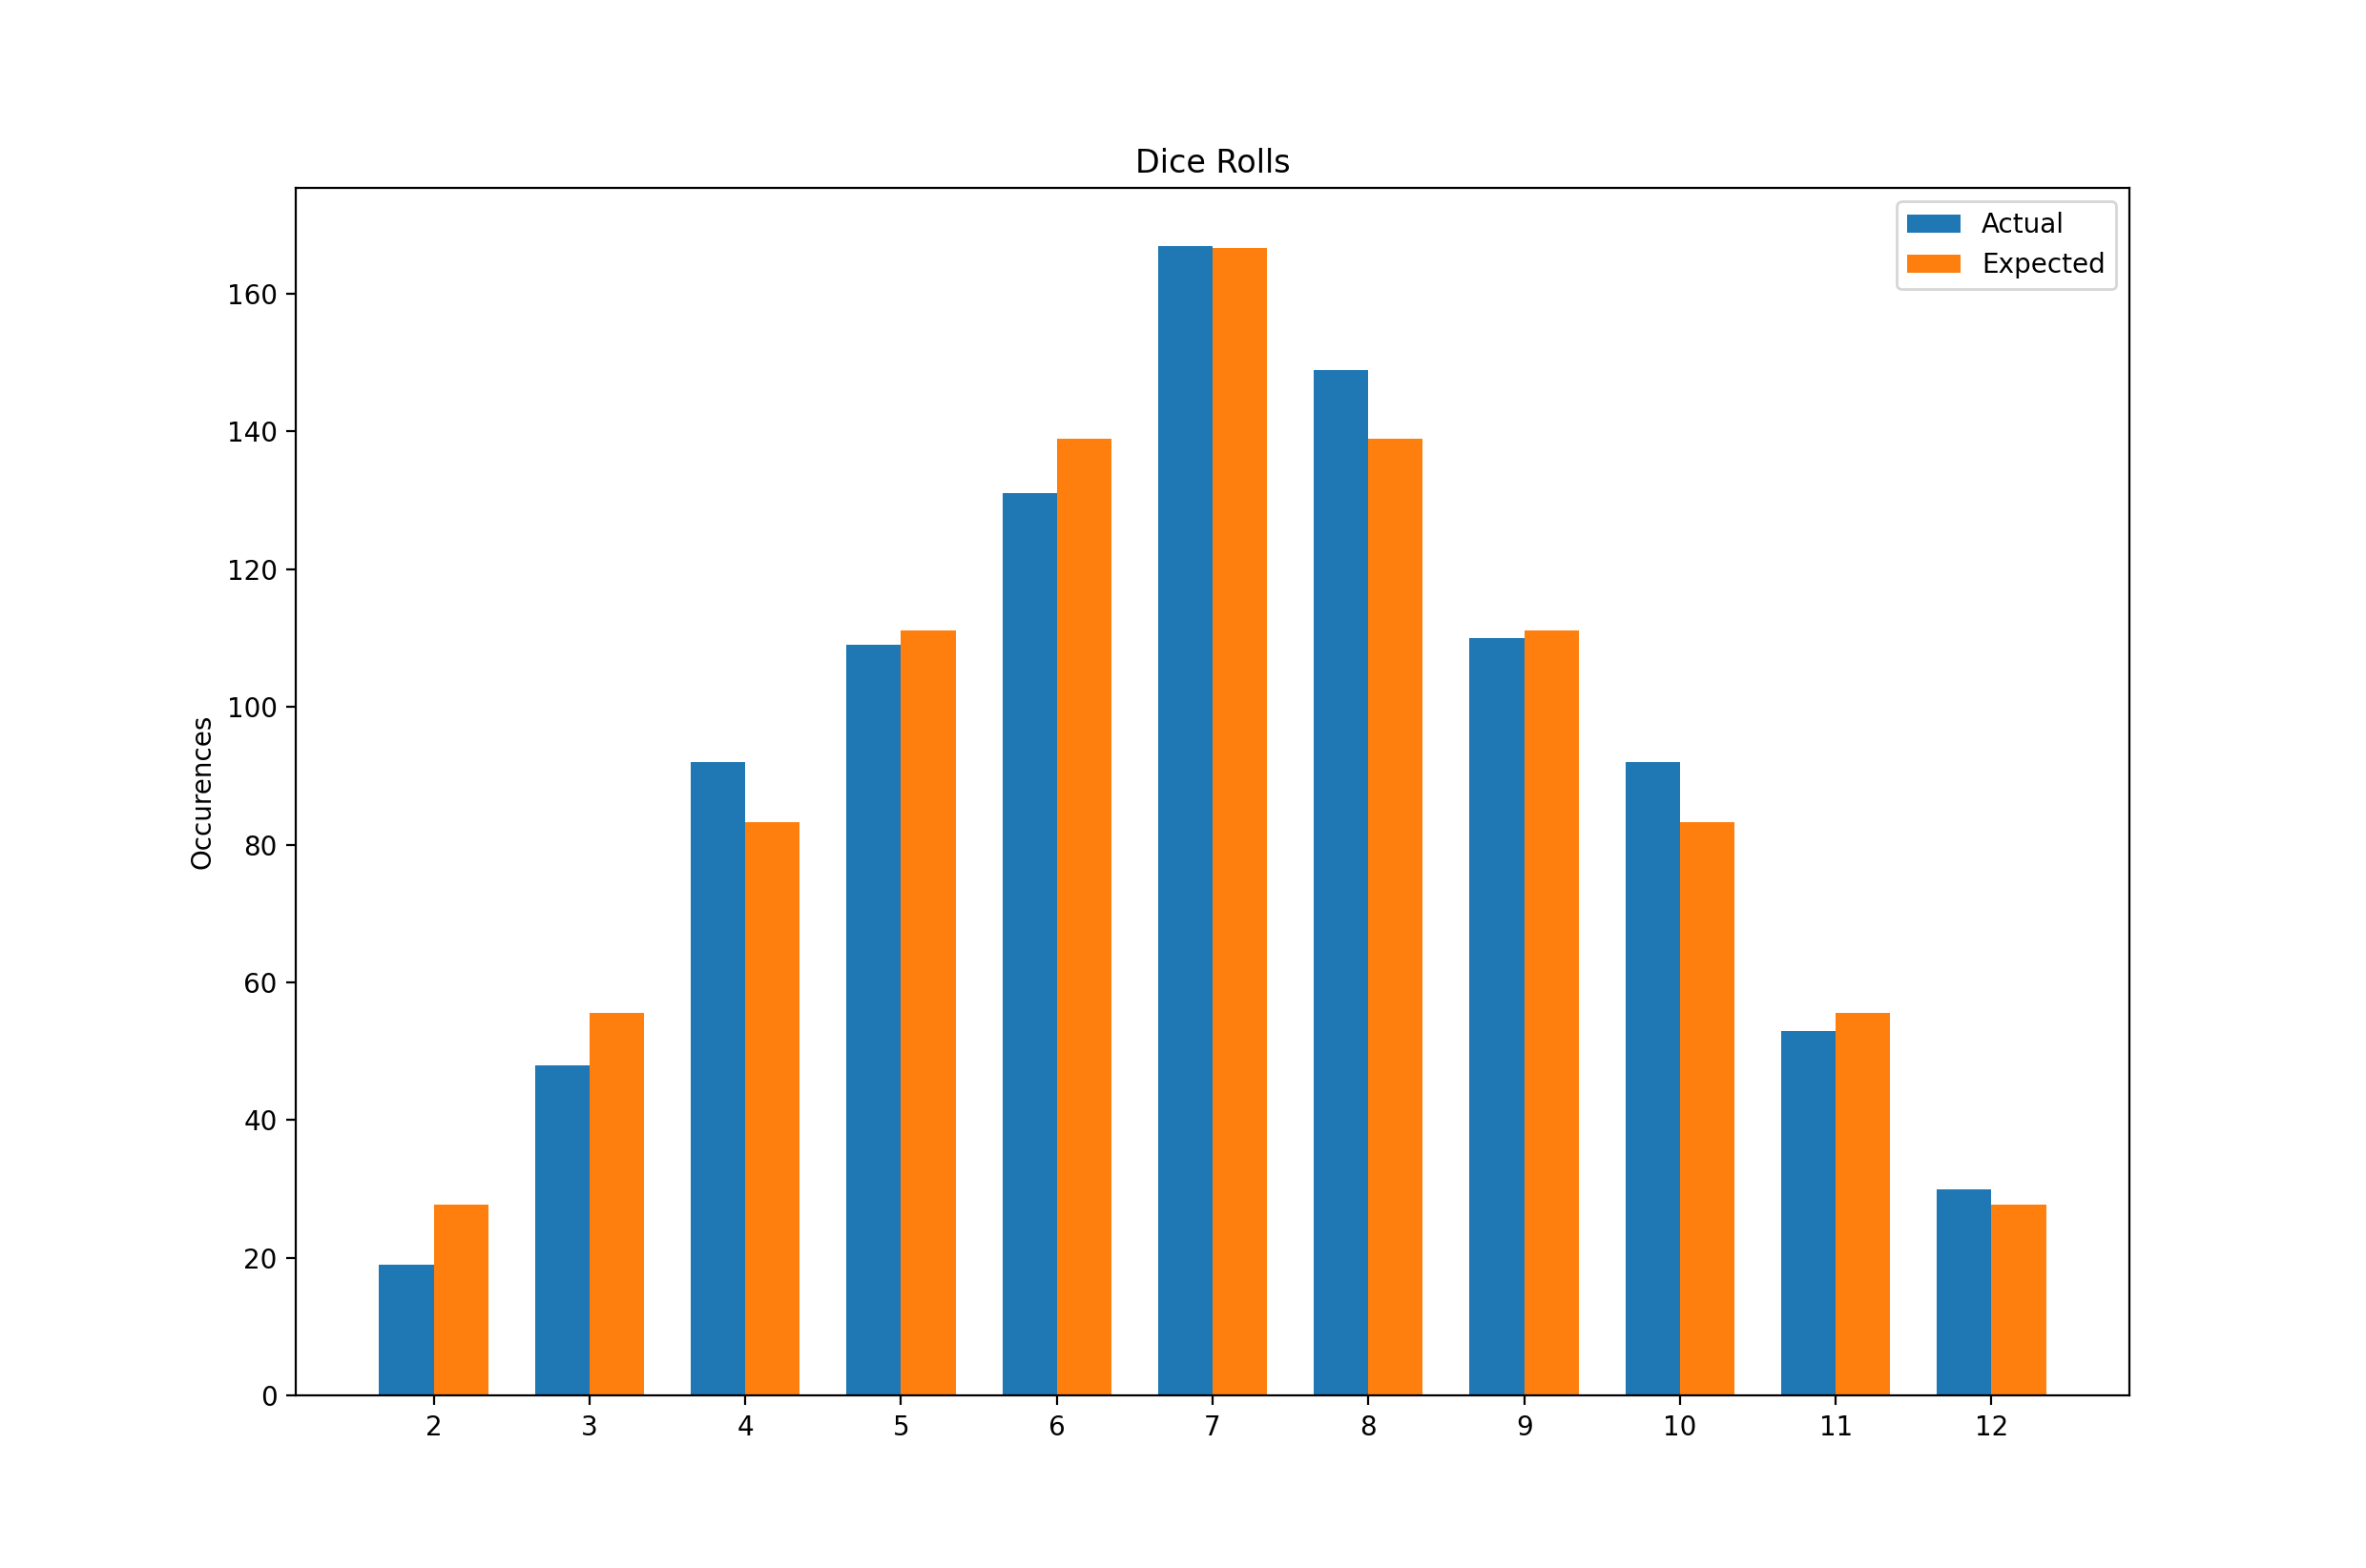
\includegraphics[width= 0.85\textwidth]{dice1.png}
    \caption{Dice roll histogram.}
    \label{fig:dice1}
\end{figure}

We need to describe the set of rectangles. To do this we will loop through each possible roll (2 - 12) and put data in four lists for each:
% ADD: Define lists
\begin{minted}{python}
import random
import matplotlib.pyplot as plt

# Can't ever be 0 or 1
p = [0.0, 0.0, 1/36, 1/18, 1/12, 1/9, 5/36, 1/6, 5/36, 1/9, 1/12, 1/18, 1/36]
roll_count = 1000

# Make an array containing 13 zeros
counts = [0] * 13

for i in range(roll_count):
    a = random.randrange(6) + 1
    b = random.randrange(6) + 1
    roll = a + b

    # Increment the count for roll
    counts[roll] += 1

# Gather data for bar chart
bar_width = 0.35
expected = []
actual_starts = []
expected_starts = []
labels = []
actual = []
for i in range(2,13):
    expected.append(p[i] * roll_count)
    actual.append(counts[i])      
    actual_starts.append(i - bar_width/2)
    expected_starts.append(i + bar_width/2)
    labels.append(i)
    
fig, ax = plt.subplots()
    
# Create the bars
ax.bar(actual_starts, actual, bar_width, label='Actual')
ax.bar(expected_starts, expected, bar_width, label='Expected')
ax.set_xticks(labels)

# Provide labels
ax.set_ylabel('Occurrences')
ax.set_title('Dice Rolls')
ax.legend()
plt.show()
\end{minted}

% ADD: For extra guidance: https://pythoniseasytolearn.blogspot.com/2019/09/rolling-two-dice.html


\section{Beginning Combinatorics}
Discrete probability problems often include some counting. For
example, we figured out that there were 36 different ways the two dice could land, 
but all of them summed to some number 2 through 12. How
many different ways could three eight-sided dice come up? We would need to
count them, right? As the numbers get bigger, we will need some tricks so that
we do not need to write them all down and count them one-by-one.

The branch of mathematics that focuses on tricks for counting is
called \textit{combinatorics}.\index{combinatorics}
% KA: https://www.khanacademy.org/computing/pixar/crowds/crowds-1/v/combinatorics1

How can we be sure that there were 36 different configurations for the
two 6-sided dice? The first die could have come up as any one of six
numbers. For each of those, the second could have come up with any one
of six numbers. Thus, the \index{multiplication principle}number of possibilities is $ 6 \times 6 =
36.$

How many different configurations for three 8-sided dice?  $8 \times 8
\times 8 = 8^3 = 512$.

What about seven dice, each with 20 sides? There would be $20^7=1,280,000,000$
configurations. See, are you glad that we do not need to write them all down?

Now, let us say that six people (Anne, Brock, Carl, Dev, Edgar, and Fred) are
going to run a race. You have to make a plaque that says who won first
place, who won second place, and who won third. If you want to get all
the possible plaques created beforehand, and just pull the right one
out as soon as the race ends, how many plaques would you need to get
engraved?

% 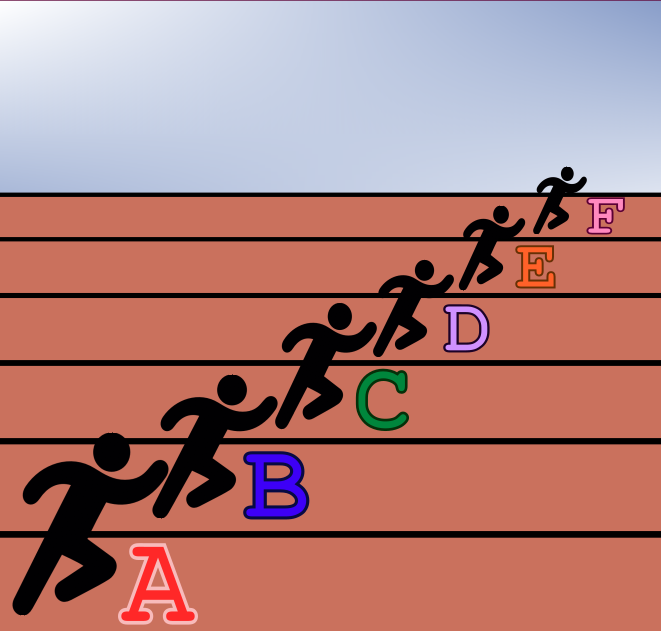
\includegraphics[width=0.8\textwidth]{Race.png}

Since you are making these plaques before the race even happens, you need one
plaque for every possible outcome. So think of it as filling in three blanks:
first place, second place, and third place. Any of the 6 people could fill
the first blank. Whoever fills that blank cannot also fill the second blank
--- a person cannot come in both first \textit{and} second --- so only 5
people are left to fill the second blank. Likewise, only 4 people remain
to fill the third blank, since two people have already been assigned to
the first two spots. Multiplying these together, $6 \times 5 \times 4 =
120$, tells you exactly how many different first-second-third outcomes
are possible --- and thus how many plaques you would need engraved.

What if the plaque includes all 6 places?  Using the same reasoning, you would
fill in six blanks instead of three: $6 \times 5 \times 4 \times 3 \times 2
\times 1 = 720$ plaques engraved.  We use this process often enough that
we gave it a name.  We say ``I need 6 factorial plaques engraved.''  When
we write a \newterm{factorial}, we use an exclamation point:\index{factorial}

$$6! = 6 \times 5 \times 4 \times 3 \times 2 \times 1 = 720$$
We use the word ``permutation'' to mean a particular ordering.
This rule says $n$ items can be ordered in $n!$ ways. Thus,
mathematicians actually say ``If you have a list of $n$ items then we
can generate $n!$ different permutations of those items.'' We will return to permutations at the end of this chapter. 

In Python, there is a \pyfunction{factorial} function in the math library:
\begin{minted}{python} 
>>> import math
>>> math.factorial(6)
720
\end{minted}

Handy, right? Now you do not need to write a loop to calculate factorials.

Remember when we only wanted the first three names on the plaque? We can solve that problem using factorials:

$$6 \times 5 \times 4 = \frac{6 \times 5 \times 4 \times 3 \times 2 \times 1}{3 \times 2 \times 1} = \frac{6!}{3!}$$

This formulation makes it easy to figure out on any calculator with a ``!'' button.

The rule on this is to fill $m$ positions from $n$ items. It can be done this many ways:
\index{permutations!formula}
\begin{mdframed}[frametitle = {Permutations}, style = important]
For permutations where order is a factor, the formula for ${}^nP_m$ ($n$ objects pick $m$) is 
$$\frac{n!}{(n-m)!}$$
\end{mdframed}
% KA: https://www.khanacademy.org/computing/pixar/crowds/crowds2/v/combinatorics8

\subsection{Choose}

Let us say that there are 12 kids in a classroom and you need a team
of four to clean the top of the desks. How many different possible teams are
there? You know that if you were giving out four different positions
(Like the race gave out 1st, 2nd, and 3rd), the answer would be $12\times 11 \times 10 \times 9$ or $12! / (12 - 4)!$.
% ADD: This is the probability that one person would be chosen

However, once we pick the 4 people, we do not care what order they are
in, right?  In this problem, the team ``Anne, Brad, Carl, and Don'' is
the same as the team ``Carl, Don, Brad, and Anne''.

Thus, the quantity $12! / (12 - 4)!$ is many times too large, because
it counts each permutation separately. To get the right number, we
just divide this by the number of possible permutations for a group of
four people: $4!$

That gets us our answer: How many different teams of four can be chosen from 12 people?

$$\frac{12!}{(12-4)! 4!}= 495$$
% ADD: Needs a bit more explanation for clarity, might just be my understanding
This number is called a \newterm{binomial coefficient}. \index{binomial coefficient}
In combinatorics, we use this quantity a lot, so we have given it a name: \textit{choose}\index{choose function}
\index{combinations!formula}
\begin{mdframed}[frametitle = {Combinations}, style = important]
For combinations, where order does not matter, the formula for ${}^n C_k$ ($n$ objects choose $k$) is 
$${n \choose k} = \frac{n!}{k!(n-k)!}$$
\end{mdframed}
We have also given it a notation. ``12 choose 4'' is written like this:

$${12 \choose 4}$$
%FIXME go more indepth on binomial distribution applied to combinatorics
% KA Binomial Theorem: https://www.khanacademy.org/math/precalculus/x9e81a4f98389efdf:series/x9e81a4f98389efdf:binomial/v/binomial-theorem

Python has the \pyfunction{math.comb} function:

\begin{minted}{python}
>>> import math
>>> math.comb(12, 4)
495  
\end{minted}

We briefly saw this in the common polynomial products chapter. The \index{binomial theorem}binomial theorem says that the coefficients of the terms in the expansion of $(a + b)^n$ are given by the binomial coefficients ${n \choose k}$.
\begin{equation*}
(a + b)^4 = 1a^4 + 4a^3b + 6a^2 b^2 + 4 a b^3 + 1 b^4 =\binom{4}{0}a^4 + \binom{4}{1}a^3b + \binom{4}{2}a^2b^2 + \binom{4}{3}ab^3 + \binom{4}{4}b^4
\end{equation*}
\subsection{Fractional Binomial Theorem}
An issue arises when we have fractional exponents for this theorem. For example, what is $\sqrt{1+5x}=(1 + 5x)^{1/2}$? We can use the binomial theorem to expand this as follows:
\begin{equation*}
(1 + 5x)^{1/2} = \binom{1/2}{0}1 + \binom{1/2}{1}5x + \binom{ 
1/2}{2}(5x)^2 + \binom{1/2}{3}(5x)^3 + \ldots
\end{equation*}
\index{Pascal's triangle}Pascal's triangle only works when the exponent $n$ is a non-negative integer. Here, the exponent is $\frac{1}{2}$, not a whole number. There is no "row $\frac{1}{2}$" of Pascal's triangle, so we need to extend the pattern.

This extension is called the \textbf{\newterm{general binomial theorem}}. To make sense of $\binom{1/2}{k}$, we need a definition of the binomial coefficient that does not rely on factorials, since $(1/2)!$ does not make sense. Recall that
\begin{equation*}
\binom{n}{k} = \frac{n!}{k!(n-k)!} = \frac{n(n-1)(n-2)\cdots(n-k+1)}{k!}
\end{equation*}
Notice that the right-hand side only ever multiplies and divides — it never actually requires $n$ to be a whole number! This gives us a definition that works for \emph{any} real number $n$, including fractions and negative numbers:
\index{binomial coefficient!generalized}
\begin{mdframed}[frametitle = {Generalized Binomial Coefficient}, style = important]
For any real number $n$ and non-negative integer $k$,
\begin{equation*}
\binom{n}{k} = \frac{n(n-1)(n-2)\cdots(n-k+1)}{k!}
\end{equation*}
\end{mdframed}

When $n$ is \emph{not} a non-negative integer, like $n = \frac{1}{2}$, none of the factors $n, n-1, n-2, \ldots$ is ever zero, so the expansion never terminates. Instead of a finite row of Pascal's triangle, we get an infinite series.

\begin{mdframed}[frametitle = {General Binomial Theorem}, style = important]
Recall that for $|x| < 1$, the \index{geometric series}geometric series gives
\begin{equation*}
    \frac{1}{1-x} = 1 + x + x^2 + x^3 + \cdots
\end{equation*}
Since $\frac{1}{1-x} = (1-x)^{-1}$, this looks like a binomial expansion where the exponent $-1$ is not a positive integer. Using the generalized binomial coefficient,
\begin{equation*}
    \binom{n}{k} = \frac{n(n-1)(n-2)\cdots(n-k+1)}{k!}
\end{equation*}
For any real number $n$ and $|x| < 1$,
\begin{equation*}
(1+x)^n = \sum_{k=0}^{\infty} \binom{n}{k}x^k = 1 + nx + \frac{n(n-1)}{2!}x^2 + \frac{n(n-1)(n-2)}{3!}x^3 + \cdots
\end{equation*}
this is called the \index{binomial series}\newterm{binomial series}, and it generalizes the binomial theorem to arbitrary real exponents. Setting $n = -1$ recovers the geometric series above.
\end{mdframed}

The condition $|x| < 1$ matters here for convergence. When $n$ was a positive integer, the expansion was just a polynomial, and polynomials are perfectly well-behaved for every value of $x$. But now that we have an infinite series, we need the terms to actually get smaller and smaller so the sum settles down to a finite value. If $|x| \geq 1$, the terms do not shrink, and the series does not converge to anything useful.

Let us compute the coefficients for $\binom{1/2}{k}$
\begin{align*}
\binom{1/2}{0} &= 1 \\
\binom{1/2}{1} &= \frac{1}{2} \\
\binom{1/2}{2} &= \frac{\frac{1}{2}\left(\frac{1}{2}-1\right)}{2!} = \frac{\frac{1}{2}\cdot\left(-\frac{1}{2}\right)}{2} = -\frac{1}{8} \\
\binom{1/2}{3} &= \frac{\frac{1}{2}\left(-\frac{1}{2}\right)\left(-\frac{3}{2}\right)}{3!} = \frac{3/8}{6} = \frac{1}{16}
\end{align*}
So,
\begin{equation*}
(1+x)^{1/2} = 1 + \frac{1}{2}x - \frac{1}{8}x^2 + \frac{1}{16}x^3 - \cdots
\end{equation*}

Now we can go back to our original problem, $\sqrt{1+5x} = (1+5x)^{1/2}$. This is just $(1+x)^{1/2}$ with $x$ replaced by $5x$, so we substitute $5x$ everywhere:
\begin{align*}
\sqrt{1+5x} &= 1 + \frac{1}{2}(5x) - \frac{1}{8}(5x)^2 + \frac{1}{16}(5x)^3 - \cdots \\
&= 1 + \frac{5}{2}x - \frac{25}{8}x^2 + \frac{125}{16}x^3 - \cdots
\end{align*}
This expansion is only valid for $|5x| < 1$, i.e. $|x| < \frac{1}{5}$.

\begin{Exercise}[title={Fractional Binomial Expansion}, label=fracbinom]
  \Question{Find the first four terms in the expansion of $(1+x)^{-1}$, in ascending powers of $x$. For what values of $x$ is this expansion valid?}
  \Question{Find the first three terms in the expansion of $\sqrt{1-2x}$, in ascending powers of $x$.}
\end{Exercise}
\begin{Answer}[ref=fracbinom]
  1. $(1+x)^{-1} = 1 - x + x^2 - x^3 + \cdots$, valid for $|x| < 1$

  2. $\sqrt{1-2x} = 1 - x - \frac{1}{2}x^2 - \cdots$
\end{Answer}
\subsection{Applications in Probability}

Suppose you flip a fair coin 5 times. What is the probability that you get exactly 3 heads? 

Note that there are only two options: Heads (H) or Tails (T). Thus, there are $2^5 = 32$ possible sequences of flips. Each sequence is equally likely, so the probability of any particular sequence is $\frac{1}{32}$. Only a certain number of sequences will have exactly 3 heads.

One way to get 3 heads is HHHTT. There is also HTHHT, THHHT, and many other orderings also give you 3 heads. Before we can find the probability, we need to know \textit{how many} different sequences of 5 coin flips contain exactly 3 heads. As we have discussed, we can use the $n$-choose-$k$ formula. There are

$$\binom{5}{3} = \frac{5!}{3!2!} = 10$$

such sequences. This is said "5 choose 3", or, more explicitly ``get 3 successes in 5 trials''. 

Each individual sequence, like HHHTT, has probability $\left(\frac{1}{2}\right)^3\left(\frac{1}{2}\right)^2$ of occurring, since each flip is independent. Since there are 10 equally likely sequences that give exactly 3 heads, we add up 10 copies of that probability:

$$P(\text{exactly 3 heads}) = \binom{5}{3}\left(\frac{1}{2}\right)^3\left(\frac{1}{2}\right)^2 = 10 \cdot \frac{1}{32} = \frac{10}{32} = \frac{5}{16}$$

This pattern of counting the arrangements with $\binom{n}{k}$, then multiplying by the probability of one arrangement works whenever you have repeated \emph{independent} trials with only two possible outcomes each time (success or failure). 

\begin{Exercise}[title={Free Throws}, label={ex:free_throw_prob}]
A basketball player has a past record of making 60\% of their free throws. Over the next 6 free throws, what is the probability that she makes exactly 4 of them?
\end{Exercise}


\begin{Answer}[ref={ex:free_throw_prob}]

\[
P(\text{exactly 4 makes}) = \binom{6}{4}(0.6)^4(0.4)^2 = 15 \times 0.1296 \times 0.16 = 0.31104
\]
About 31\%.

\end{Answer}
This probability situation has been rightfully called the \index{binomial distribution}\newterm{binomial distribution}. This is a brief introduction to the binomial distribution, and we will discuss it in more detail in a later chapter.


\section{Permutations and Sorting}
We counted permutations earlier in this chapter. If you have a list
of four letters, like $[a, b, c, d]$, you can rearrange them in $4!$
ways:\index{permutations}

\begin{tabular}{c c c c c c}
  a,b,c,d & a,b,d,c & a, d, b, c & a, d, c, b & a, c, b, d & a, c, d, b \\
  b,a,c,d & b,a,d,c & b, d, a, c & b, d, c, a & b, c, a, d & b, c, d, a \\
  c,b,a,d & c,b,d,a & c, d, b, a & c, d, a, b & c, a, b, d & c, a, d, b \\
  d,b,c,a & d,b,a,c & d, a, b, c & d, a, c, b & d, c, b, a & d, c, a, b
\end{tabular}
% KA: https://www.khanacademy.org/math/precalculus/x9e81a4f98389efdf:prob-comb/x9e81a4f98389efdf:combinations/v/combination-formula

You can make Python generate all the permutations for you:

\begin{minted}{python}
from itertools import permutations
all_permutations = permutations(('a', 'b', 'c', 'd'))
for p in all_permutations:
    print(p)
\end{minted}
% KA: https://www.khanacademy.org/math/precalculus/x9e81a4f98389efdf:prob-comb/x9e81a4f98389efdf:combinations/v/introduction-to-combinations

\subsection{Notation}

How do we define or write down a single permutation? You could say
something like ``Swap the first and second items and swap the third
and fourth items.'' However, that gets pretty difficult to read, so we
usually write a permutation as two lines: the first line is before
the permutation and the second line is after.  Like this:

$$\begin{pmatrix}
  1 & 2 & 3 & 4 \\
  2 & 1 & 4 & 3
\end{pmatrix}$$

We can also assign permutations to variables. For example, if we wanted the
variable $A$ to represent ``swapping the first and second item'', we
would write this:

$$A = \begin{pmatrix}
  1 & 2 & 3 & 4 \\
  2 & 1 & 3 & 4
\end{pmatrix}$$

And if we wanted $B$ to represent ``swapping the third and fourth item'', we would write:

$$B = \begin{pmatrix}                                                                                                                             
  1 & 2 & 3 & 4 \\                                                                                                                                
  1 & 2 & 4 & 3
\end{pmatrix}$$

Now, we can \textit{compose} permutations together. For example, we might say:\index{permutations!composing}

$$B \circ A = \begin{pmatrix}
  1 & 2 & 3 & 4 \\
  2 & 1 & 4 & 3
\end{pmatrix}$$

In other words, if we have the list $[a, b, c, d]$ and we apply permutation $A$, followed by permutation $B$, we get $[b, a, d, c]$.

\textbf{Important:} Note that permutations are applied from right to
left. $B \circ A$ means ``Applying $A$ and then $B$.''  Why does this matter?
Permutations are not necessarily \index{commutativity}commutative. That is, if you have two
permutations $S$ and $T$, $S \circ T$ is not always the same as $T
\circ S$.

Also, note that ``do not change anything'' is a permutation. We call it
\textit{the identity permutation}. If you have four items, the identity
permutation would be written:\index{permutations!identity permutation}

$$I = \begin{pmatrix}
  1 & 2 & 3 & 4 \\
  1 & 2 & 3 & 4
\end{pmatrix}$$

(We use a capital ``I'' for the identity.)

\subsubsection{Challenge} Find an example of two permutations $S$ and $T$, such that $S \circ T$ does not equal $T \circ S$.

Hint: on a list of three items, try swapping the first two items and swapping the last two items.

(One answer: let $S$ swap positions 1 and 2, and $T$ swap positions 2 and 3. Starting from $[a, b, c]$, $S \circ T$ gives $[c, a, b]$, but $T \circ S$ gives $[b, c, a]$.)

\subsection{Sorting in Python}

One of the common forms of permutation in software is sorting.
Sorting is putting data in a particular order. For example, in Python,
if you had a list of numbers, you can sort it in ascending order like
this:\index{sorting}

\begin{minted}{python}
my_grades = [92, 87, 76, 99, 91, 93]
grades_worst_to_best = sorted(my_grades)
\end{minted}

Do you want to sort backwards?

\begin{minted}{python}
my_grades = [92, 87, 76, 99, 91, 93]
grades_best_to_worst = sorted(my_grades, reverse=True)
\end{minted}

Note that \pyfunction{sorted} \index{sorted()}makes a new list with the correct
order. If you want to sort the array in place, you can use the
\pyfunction{sort} method:
% ADD: Need to define array

\begin{minted}{python}
my_grades = [92, 87, 76, 99, 91, 93]
my_grades.sort(reverse=True)
\end{minted}

\subsection{Inverses}

Think for a second about this permutation:

$$S = \begin{pmatrix}
  1 & 2 & 3 & 4 \\
  3 & 4 & 2 & 1
\end{pmatrix}$$

You could say this permutation shuffles a list.  What is its
inverse? That is, what is the permutation that unshuffles the items
back to where they were originally?\index{permutations!inverses}

$$S^{-1} = \begin{pmatrix}
  1 & 2 & 3 & 4 \\
  4 & 3 & 1 & 2
\end{pmatrix}$$

In other words, the original moved an item in the first spot to the third
spot; the inverse must move whatever was in the third spot back to
the first spot.

(Notation note: In multiplication, $b \times b^{-1} = 1$, so we
use ``to the negative one'' to indicate inverses in lots of places.)

Mechanically, how do you find the inverse? Flip the rows, then sort the columns using the top number:
% ADD: Inverse should probably be defined
$$\begin{pmatrix}
  1 & 2 & 3 & 4 \\
  3 & 4 & 2 & 1
\end{pmatrix}
\text{ flip }\rightarrow
\begin{pmatrix}
  3 & 4 & 2 & 1 \\
  1 & 2 & 3 & 4
\end{pmatrix}
\text{ sort }\rightarrow
\begin{pmatrix}
  1 & 2 & 3 & 4 \\
  4 & 3 & 1 & 2
\end{pmatrix}
$$    

Let us say you have two permutations $A$ and $B$. Permuting by $B$ then $A$ would look like this:

$$C = A \circ B$$

If you know $A^{-1}$ and $B^{-1}$, what is $C^{-1}$?  You would undo-$A$, then undo-$B$, so

$$C^{-1} = B^{-1} \circ A^{-1}$$

\subsection{Cycles}

Here is a permutation:

$$\begin{pmatrix}
  1 & 2 & 3 & 4 & 5 \\
  2 & 4 & 5 & 1 & 3
\end{pmatrix}$$

When this is applied, whatever is at 1 gets moved to 2, 2 gets moved
to 4, and 4 gets moved to 1.  That is a \index{cycle}\textit{cycle}: $1 \rightarrow
2 \rightarrow 4$, then it goes back to 1. It involves three locations, so we say
it is a \textit{3-cycle}.\index{permutations!cycles}

There is another cycle in this permutation: $3 \rightarrow 5$, then it goes back to 3.

Because these cycles share no members, we say the cycles are \index{disjoint cycles}\textit{disjoint}.

Every permutation can be broken down into a collection of disjoint cycles.

$$T = \begin{pmatrix}
  1 & 2 & 3 & 4 & 5 \\
  2 & 4 & 5 & 1 & 3
\end{pmatrix} = (1 \rightarrow 2 \rightarrow 4)(3 \rightarrow 5)$$

The first handy thing about this notation is that it makes it easy for
us to describe the inverse. We just run the cycles backward:

$$T^{-1} = (4 \rightarrow 2 \rightarrow 1)(5 \rightarrow 3)$$

Starting with the list $[a, b, c, d, e]$, let us repeatedly apply the permutation $T$

\begin{tabular}{r | l}
  Initial & {\color{red} a, b,} {\color{blue} c,} {\color{red} d,} {\color{blue} e} \\ 
  $T$ applied & {\color{red} d, a,}  {\color{blue} e,} {\color{red} b,} {\color{blue} c}\\
  $T \circ T$ applied & {\color{red} b, d,} {\color{blue} c,} {\color{red} a,}  {\color{blue} e} \\
  $T \circ T \circ T$ applied & {\color{red} a, b,}  {\color{blue} e,} {\color{red} d,} {\color{blue} c} \\
  $T \circ T \circ T \circ T$ applied & {\color{red} d, a,} {\color{blue} c,} {\color{red}b,}  {\color{blue} e} \\
  $T \circ T \circ T \circ T \circ T$ applied & {\color{red} b, d,}  {\color{blue} e,} {\color{red} a,} {\color{blue} c} \\
  $T \circ T \circ T \circ T \circ T \circ T$ applied & {\color{red} a, b,} {\color{blue} c,} {\color{red} d,}  {\color{blue} e}\\
\end{tabular}

After six applications, the list is back where it started. The number of
applications needed, called the \newterm{order} of the permutation, is the
\index{least common multiple}least common multiple of the cycle lengths.  In this case, there is a 3-cycle and a 2-cycle. The
least common multiple of 2 and 3 is 6.

\subsection{Further Learning}
Check out this leetcode problem which combines permutations and programming! 
\url{https://leetcode.com/problems/permutations/description/}
%FIXME this chapter needs more examples and applications of permutation problems
